% Options for packages loaded elsewhere
\PassOptionsToPackage{unicode}{hyperref}
\PassOptionsToPackage{hyphens}{url}
\PassOptionsToPackage{dvipsnames,svgnames,x11names}{xcolor}
%
\documentclass[
  letterpaper,
  DIV=11,
  numbers=noendperiod]{scrartcl}

\usepackage{amsmath,amssymb}
\usepackage{lmodern}
\usepackage{iftex}
\ifPDFTeX
  \usepackage[T1]{fontenc}
  \usepackage[utf8]{inputenc}
  \usepackage{textcomp} % provide euro and other symbols
\else % if luatex or xetex
  \usepackage{unicode-math}
  \defaultfontfeatures{Scale=MatchLowercase}
  \defaultfontfeatures[\rmfamily]{Ligatures=TeX,Scale=1}
\fi
% Use upquote if available, for straight quotes in verbatim environments
\IfFileExists{upquote.sty}{\usepackage{upquote}}{}
\IfFileExists{microtype.sty}{% use microtype if available
  \usepackage[]{microtype}
  \UseMicrotypeSet[protrusion]{basicmath} % disable protrusion for tt fonts
}{}
\makeatletter
\@ifundefined{KOMAClassName}{% if non-KOMA class
  \IfFileExists{parskip.sty}{%
    \usepackage{parskip}
  }{% else
    \setlength{\parindent}{0pt}
    \setlength{\parskip}{6pt plus 2pt minus 1pt}}
}{% if KOMA class
  \KOMAoptions{parskip=half}}
\makeatother
\usepackage{xcolor}
\setlength{\emergencystretch}{3em} % prevent overfull lines
\setcounter{secnumdepth}{-\maxdimen} % remove section numbering
% Make \paragraph and \subparagraph free-standing
\ifx\paragraph\undefined\else
  \let\oldparagraph\paragraph
  \renewcommand{\paragraph}[1]{\oldparagraph{#1}\mbox{}}
\fi
\ifx\subparagraph\undefined\else
  \let\oldsubparagraph\subparagraph
  \renewcommand{\subparagraph}[1]{\oldsubparagraph{#1}\mbox{}}
\fi


\providecommand{\tightlist}{%
  \setlength{\itemsep}{0pt}\setlength{\parskip}{0pt}}\usepackage{longtable,booktabs,array}
\usepackage{calc} % for calculating minipage widths
% Correct order of tables after \paragraph or \subparagraph
\usepackage{etoolbox}
\makeatletter
\patchcmd\longtable{\par}{\if@noskipsec\mbox{}\fi\par}{}{}
\makeatother
% Allow footnotes in longtable head/foot
\IfFileExists{footnotehyper.sty}{\usepackage{footnotehyper}}{\usepackage{footnote}}
\makesavenoteenv{longtable}
\usepackage{graphicx}
\makeatletter
\def\maxwidth{\ifdim\Gin@nat@width>\linewidth\linewidth\else\Gin@nat@width\fi}
\def\maxheight{\ifdim\Gin@nat@height>\textheight\textheight\else\Gin@nat@height\fi}
\makeatother
% Scale images if necessary, so that they will not overflow the page
% margins by default, and it is still possible to overwrite the defaults
% using explicit options in \includegraphics[width, height, ...]{}
\setkeys{Gin}{width=\maxwidth,height=\maxheight,keepaspectratio}
% Set default figure placement to htbp
\makeatletter
\def\fps@figure{htbp}
\makeatother
\newlength{\cslhangindent}
\setlength{\cslhangindent}{1.5em}
\newlength{\csllabelwidth}
\setlength{\csllabelwidth}{3em}
\newlength{\cslentryspacingunit} % times entry-spacing
\setlength{\cslentryspacingunit}{\parskip}
\newenvironment{CSLReferences}[2] % #1 hanging-ident, #2 entry spacing
 {% don't indent paragraphs
  \setlength{\parindent}{0pt}
  % turn on hanging indent if param 1 is 1
  \ifodd #1
  \let\oldpar\par
  \def\par{\hangindent=\cslhangindent\oldpar}
  \fi
  % set entry spacing
  \setlength{\parskip}{#2\cslentryspacingunit}
 }%
 {}
\usepackage{calc}
\newcommand{\CSLBlock}[1]{#1\hfill\break}
\newcommand{\CSLLeftMargin}[1]{\parbox[t]{\csllabelwidth}{#1}}
\newcommand{\CSLRightInline}[1]{\parbox[t]{\linewidth - \csllabelwidth}{#1}\break}
\newcommand{\CSLIndent}[1]{\hspace{\cslhangindent}#1}

\usepackage{amsmath}
\usepackage{booktabs}
\usepackage{caption}
\usepackage{longtable}
\KOMAoption{captions}{tableheading}
\makeatletter
\makeatother
\makeatletter
\makeatother
\makeatletter
\@ifpackageloaded{caption}{}{\usepackage{caption}}
\AtBeginDocument{%
\ifdefined\contentsname
  \renewcommand*\contentsname{Table of contents}
\else
  \newcommand\contentsname{Table of contents}
\fi
\ifdefined\listfigurename
  \renewcommand*\listfigurename{List of Figures}
\else
  \newcommand\listfigurename{List of Figures}
\fi
\ifdefined\listtablename
  \renewcommand*\listtablename{List of Tables}
\else
  \newcommand\listtablename{List of Tables}
\fi
\ifdefined\figurename
  \renewcommand*\figurename{Figure}
\else
  \newcommand\figurename{Figure}
\fi
\ifdefined\tablename
  \renewcommand*\tablename{Table}
\else
  \newcommand\tablename{Table}
\fi
}
\@ifpackageloaded{float}{}{\usepackage{float}}
\floatstyle{ruled}
\@ifundefined{c@chapter}{\newfloat{codelisting}{h}{lop}}{\newfloat{codelisting}{h}{lop}[chapter]}
\floatname{codelisting}{Listing}
\newcommand*\listoflistings{\listof{codelisting}{List of Listings}}
\makeatother
\makeatletter
\@ifpackageloaded{caption}{}{\usepackage{caption}}
\@ifpackageloaded{subcaption}{}{\usepackage{subcaption}}
\makeatother
\makeatletter
\@ifpackageloaded{tcolorbox}{}{\usepackage[many]{tcolorbox}}
\makeatother
\makeatletter
\@ifundefined{shadecolor}{\definecolor{shadecolor}{rgb}{.97, .97, .97}}
\makeatother
\makeatletter
\makeatother
\ifLuaTeX
  \usepackage{selnolig}  % disable illegal ligatures
\fi
\IfFileExists{bookmark.sty}{\usepackage{bookmark}}{\usepackage{hyperref}}
\IfFileExists{xurl.sty}{\usepackage{xurl}}{} % add URL line breaks if available
\urlstyle{same} % disable monospaced font for URLs
\hypersetup{
  pdftitle={Assignment 5},
  colorlinks=true,
  linkcolor={blue},
  filecolor={Maroon},
  citecolor={Blue},
  urlcolor={Blue},
  pdfcreator={LaTeX via pandoc}}

\title{Assignment 5}
\author{}
\date{}

\begin{document}
\maketitle
\ifdefined\Shaded\renewenvironment{Shaded}{\begin{tcolorbox}[frame hidden, enhanced, borderline west={3pt}{0pt}{shadecolor}, interior hidden, breakable, sharp corners, boxrule=0pt]}{\end{tcolorbox}}\fi

\hypertarget{introduksjon}{%
\subsection{Introduksjon}\label{introduksjon}}

I utrente personer som begynner med styrketrening varierer økningen i
muskelstyrke, målt som 1RM, med 1\% per økt, men med en variasjon på
hele 0.1-3\% (McDonagh \& Davies, 1984), og tverrsnittet til de
styrketrente musklene øker 0.1-0.5\% per økt (Wernbom et al., 2007). Den
store varisjonen i styrke- og muskelvekst er sannsynligvis avhengig av
hvilken muskelgruppe som trenes, fibertypesammensetning, antall serier,
repetisjoner, intensitet, pausetid og genetiske ulikheter (Raastad,
2010; Tønnessen \& Rønnestad, 2018; Wackerhage, 2014).

Sannsynligvis er det et dose-respons-forhold mellom treningsmengde og
styrkeøkning per tidsenhet (Raastad, 2010). Treningsmengden er både
avhengig av antall økter i uka og hvor mange serier eller øvelser vi
trener på hver muskegruppe. Ettersom tidsbegrensninger ofte hindrer
deltakere i treningsprogrammer (Choi et al., 2017) er det av interesse å
finne den minimale treningsdosen som gir gunstige adaptasjoner.
Oversiktsarikler fra en amerikansk forskergruppe løfter konseptet om at
en serie i hver øvelse er den mest effektive treningsformen (Carpinelli,
2002; Carpinelli \& Otto, 1998). Videre hevder de at det er bortkastet
tid å gjennomføre mer enn en serie på en muskelgruppe. Andre
meta-analyser viser at moderate treningsvolum (3 serier) er fordelaktig
(Krieger, 2010, 2009). Disse ambivalente resultatene skyldes til dels
denne store interindivid-variasjonen i treningsrespons. Intraindivide
studiedesign med unilateral treningsvolum på ekstremitetene vil trolig
fjerne mye usikkerhet.

Målet med denne studien var å undersøke effekten av singel- og
multiserie (3 serier) treningsprotokoller på muskelstyrke og muskelmasse
med et intraindivid studiedesign.

\hypertarget{metode}{%
\subsection{Metode}\label{metode}}

\hypertarget{deltakere-og-studiedesign}{%
\subsubsection{Deltakere og
studiedesign}\label{deltakere-og-studiedesign}}

41 menn og kvinner deltakere ble rekrutert til den nåværende studien med
initielle kriterier som ikke-røykene og alder mellom 18 og 40 år.
Eksklusjonskriteriene var intoleranse til lokal bedøvelse, mer enn en
ukentlig styrketreningsøkt det siste året, redusert muskelstyrke pga
tidligere eller nåværende skader, og intak av medikamenter som kan
påvirke adaptasjoner til trening. I dataanalysen ble alle deltakere som
ikke gjennomførte kneekstensjonsstesting på hvert tidspunkt brukt (N =
22). Deltakernes karakteristikker vises i Table~\ref{tbl-kar}.

\hypertarget{tbl-kar}{}
\setlength{\LTpost}{0mm}
\begin{longtable}{cr}
\caption{\label{tbl-kar}Karakteristikker av deltakerne ved pretest }\tabularnewline

\toprule
 & gj.snitt (SD) \\ 
\midrule
N & 19 \\ 
Alder & 21.9 (1.49) \\ 
Kroppslengde & 178 (9.56) \\ 
Kroppsvekt & 71.8 (11) \\ 
Fettfri Masse & 9.07 (1.9) \\ 
1RM Kneekstensjon & 58.4 (13.8) \\ 
\bottomrule
\end{longtable}
\begin{minipage}{\linewidth}
Forkortelser: lean.mass, fettfri masse; load, 1RM kneekstensjon\\
\end{minipage}

Intervensjonen bestå av 12 uker med helkropp styrketrening, alle
deltakerne gjennomførte intervensjonen i løpet av september til
november. Bein-øvelser ble utført unilateralt for å tillate
innen-deltaker forskjeller i treningsvolum. Videre ble beinene til
deltakerne tilfeldig fordelt til å utføre enten en serie (1 serie
gruppen) og tre serier (3 serier gruppen), hver deltaker gjennomførte
dermed begge protokollene. Maksimal muskelstyrke i kneekstensjon ble
testet før (pre), underveis (uke 3, 5 og 9) og etter (post)
intervensjonen. Kroppssammensetning ble målt før og etter
treningsintervensjonen.

\hypertarget{dxa}{%
\subsubsection{DXA}\label{dxa}}

Kroppssammensetning ble bestemt før og etter intervensjonen med bruk av
dual-energy X-ray absorptiometry (DXA) (Lunar Prodigy, GE Healthcare,
Oslo, Norge), iht standard protokoll. Før DXA målinger ble deltakerne
bedt om å være fastende i minimum to timer og frastå all fysisk
anstrengende aktivitet de siste 48 timene. Mellom DXA målinger og
forrige stykeøkt var det to dager.

\hypertarget{maksimal-styrke-i-kneekstensjon}{%
\subsubsection{Maksimal Styrke i
kneekstensjon}\label{maksimal-styrke-i-kneekstensjon}}

Maksimal stykre i kneekstensjon ble målt som den høyeste repetisjonen
(1RM) i en unilateral kneekstensjon. Testprotokollen begynte med en
spesifikk oppvarming bestående av 10, 6 og 3 repetisjoner på 50, 75 og
85\% av predikert 1RM. Deretter ble 1RM fundet ved å øke motstanden (kg)
progresivt inntil vekten ikke ble løftet i hele bevegelsesbanen, den
høyeste vekten med fult bevegelsesutslag ble definert som 1RM. Hver
deltaker fikk 4-6 forsøk.

\hypertarget{dataanalyse-og-statistikk}{%
\subsubsection{Dataanalyse og
Statistikk}\label{dataanalyse-og-statistikk}}

All beskrvende data er presentert som gj.snitt (standardfeil) om annet
ikke er spesifisert. For å undersøke effekten av treningsvolum på
muskelhypertrofi og styrke ble det brukt mixed linear models (LLMs)
spesifisert med tid og tid til treningsvolum interaksjoner som fikserte
effekter. LMMs ble spesifisert med tilfeldige intercepts for deltakerne.
Plotter med residualer mot predikerte verdier ble visuelt inspisert for
antakelser om homoskedastisitet. Statistisk signifikansnivå ble satt til
\textless{} 0.05.

\hypertarget{resultat}{%
\subsection{Resultat}\label{resultat}}

Både singel og multipel treningssett økte muskelstyrken i 1RM
kneekstensjon Figure~\ref{fig-str}. Det ble imidlertidig ikke observert
en effekt av treningsvolum på utvikling i 1RM kneekstensjon etter 12
uker med styrketrening Table~\ref{tbl-str}.

\begin{figure}

{\centering 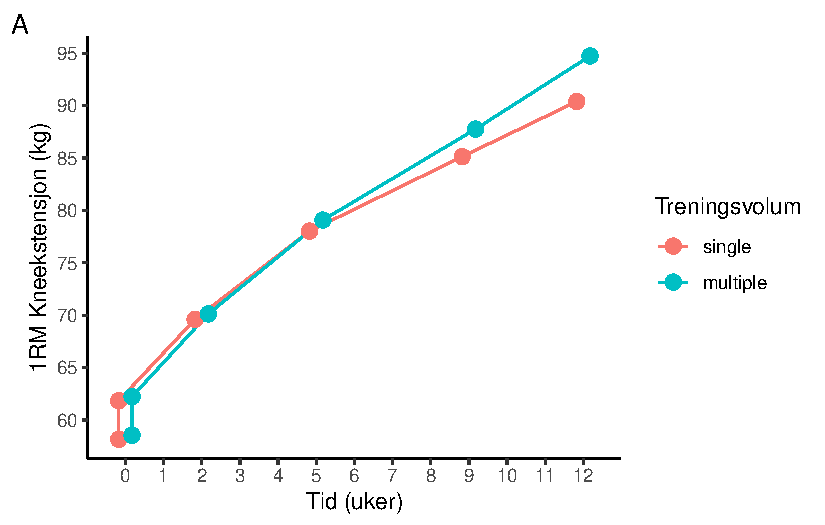
\includegraphics{assignment-5_files/figure-pdf/fig-str-1.pdf}

}

\caption{\label{fig-str}Volumavhengig effekt på muskelstyrke}

\end{figure}

\hypertarget{tbl-inc}{}
\setlength{\LTpost}{0mm}
\begin{longtable}{crrrrrr}
\caption{\label{tbl-inc}Effekten av styrketrening på muskelstyrke }\tabularnewline

\toprule
 & \multicolumn{6}{c}{Tidspunkt} \\ 
\cmidrule(lr){2-7}
Treningsvolum & Pretest & Trening 1 & Uke 2 & Uke 5 & Uke 9 & Posttest \\ 
\midrule
single & 58.2 (13.4) & 61.8 (14.2) & 69.6 (17.1) & 78 (20.8) & 85.1 (24) & 90.4 (22.9) \\ 
multiple & 58.6 (14.6) & 62.2 (16.7) & 70.1 (20.2) & 79.1 (21.7) & 87.8 (24.6) & 94.7 (26.6) \\ 
\bottomrule
\end{longtable}
\begin{minipage}{\linewidth}
Data er presenter som gj.snitt (standardfeil)\\
\end{minipage}

\hypertarget{tbl-str}{}
\setlength{\LTpost}{0mm}
\begin{longtable}{lrrrrr}
\caption{\label{tbl-str}Volumavhengig effekt på muskelstyrke fra LMM }\tabularnewline

\toprule
Koeffisienter & estimat & se & df & t.verdi & p.verdi \\ 
\midrule
Intercept & $62.05$ & $4.47$ & $19.24$ & $13.87$ & $0.00$ \\ 
Tid & $2.53$ & $0.14$ & $206.00$ & $17.71$ & $0.00$ \\ 
Gruppe3serier & $0.10$ & $1.32$ & $206.00$ & $0.08$ & $0.94$ \\ 
Tid:Gruppe3serier & $0.31$ & $0.20$ & $206.00$ & $1.54$ & $0.12$ \\ 
\bottomrule
\end{longtable}
\begin{minipage}{\linewidth}
Forkortelser: se, standardfeil; df, frihetsgrader\\
\end{minipage}

Både singel og multipel treningssett økte fettfri masse etter
treningsintervensjonen Figure~\ref{fig-lbm}. Det ble imidlertidig ikke
observert en effekt av treningsvolum på økning i fettfri masse, se
Table~\ref{tbl-lbm} og Figure~\ref{fig-lbm}.

\hypertarget{tbl-lbm}{}
\setlength{\LTpost}{0mm}
\begin{longtable}{lrrrrr}
\caption{\label{tbl-lbm}Volumavhegig effekt på muskelmasse fra LMM }\tabularnewline

\toprule
Koeffisienter & estimat & se & df & t.verdi & p.verdi \\ 
\midrule
Intercept & $9.04$ & $0.46$ & $18.37$ & $19.58$ & $0.00$ \\ 
Tid & $0.15$ & $0.08$ & $54.00$ & $2.03$ & $0.05$ \\ 
Gruppe3serier & $0.05$ & $0.08$ & $54.00$ & $0.67$ & $0.50$ \\ 
Tid:Gruppe3serier & $0.12$ & $0.11$ & $54.00$ & $1.07$ & $0.29$ \\ 
\bottomrule
\end{longtable}
\begin{minipage}{\linewidth}
Forkortelser: se, standardfeil; df, frihetsgrader\\
\end{minipage}

\begin{figure}

{\centering 

\begin{figure}

{\centering 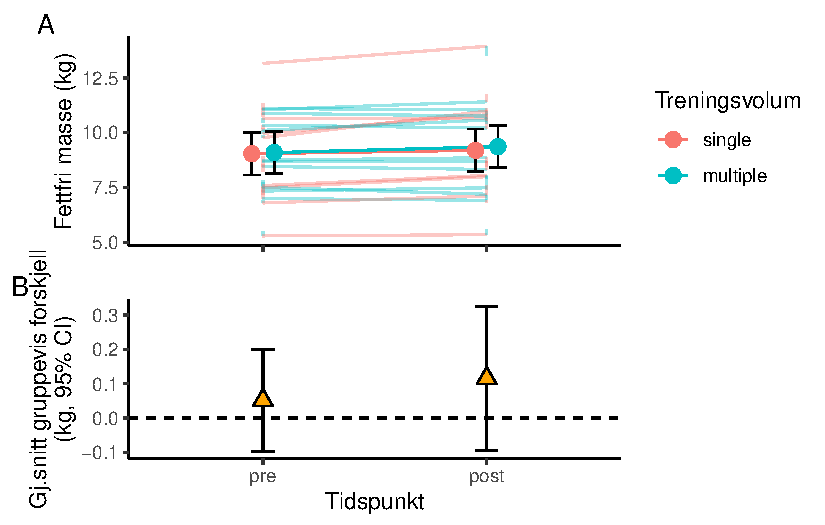
\includegraphics{assignment-5_files/figure-pdf/fig-lbm-1.pdf}

}

\caption{Figur A viser endring i fettfri masse fra pre- til posttest for
begge volumgruppene. Figur B viser den gjennomsnittlige forskjellen
mellom volumgruppene for både pre- og posttest}

\end{figure}

}

\caption{\label{fig-lbm}Volumavhengig effekt på muskelmasse}

\end{figure}

\hypertarget{diskusjon}{%
\subsection{Diskusjon}\label{diskusjon}}

I denne studien så vi ikke en effekt av treningsvolum på utvikling i
muskemasse eller muskelstyrke. For utrente individer ser det dermed ut
som man får like stor styrke- og muskelvekst av å gjennomføre en serie
per muskelgruppe som å gjennomføre tre serier. Dette samsvarer med
oversiktsartiklene som hevder at det ikke finnes en ytterligere gevinst
av å øke treningsvolumet utover en serie (Carpinelli, 2002; Carpinelli
\& Otto, 1998). Det samsvarer derimot ikke med meta-analyser som har
konkludert med at moderat volum er fordelaktig på utvikling i
muskelstyrke og muskelmasse (Krieger, 2010, 2009; Schoenfeld et al.,
2017). Resultatene i denne studien bør imidlertidig tolkes forsiktig
ettersom en nokså lav utvalgstørrelse på 19 senker den statistiske
styrken. I tillegg var deltakerne på et lavt treningsnivå før
treningsintervensjonen, dette er av betydning ettersom at effekten av
treningsvolum på styrke- og muskelvekst er trolig lavere for utrente
(Raastad, 2010). Generelt ser det ut til at jo bedre trent personen er,
desto flere serier må personen trene på hver muskelgruppe (Peterson et
al., 2004; Rhea et al., 2003).

\hypertarget{konklusjon}{%
\subsubsection{Konklusjon}\label{konklusjon}}

Denne studien indikerer at det for utrente ikke finnes en effekt av
treningsvolum (1 serie vs 3 serier) på styrke- og muskelvekst på 12
ukers treningsprogram. Dette viser at gunstige treningsadaptasjoner
oppstår på minimale treningsvolum som en serie per muskelgruppe.
Resultatene bør allikevel tolkes noe forsiktet da det er noen
metedologiske svakheter i studien, bl.a lav utvalgstørrelse og lav
treningsstatus.

\hypertarget{referanser}{%
\subsection*{Referanser}\label{referanser}}
\addcontentsline{toc}{subsection}{Referanser}

\hypertarget{refs}{}
\begin{CSLReferences}{1}{0}
\leavevmode\vadjust pre{\hypertarget{ref-carpinelli_berger_2002}{}}%
Carpinelli, R. N. (2002). Berger in retrospect: Effect of varied weight
training programmes on strength. \emph{British Journal of Sports
Medicine}, \emph{36}(5), 319--324.
\url{https://doi.org/10.1136/bjsm.36.5.319}

\leavevmode\vadjust pre{\hypertarget{ref-carpinelli_strength_1998}{}}%
Carpinelli, R. N., \& Otto, R. M. (1998). Strength {Training}: {Single}
{Versus} {Multiple} {Sets}. \emph{Sports Medicine}, \emph{26}(2),
73--84. \url{https://doi.org/10.2165/00007256-199826020-00002}

\leavevmode\vadjust pre{\hypertarget{ref-choi_correlates_2017}{}}%
Choi, J., Lee, M., Lee, J., Kang, D., \& Choi, J.-Y. (2017). Correlates
associated with participation in physical activity among adults: A
systematic review of reviews and update. \emph{BMC Public Health},
\emph{17}(1), 356. \url{https://doi.org/10.1186/s12889-017-4255-2}

\leavevmode\vadjust pre{\hypertarget{ref-krieger_single_2010}{}}%
Krieger, J. W. (2010). Single vs. {Multiple} {Sets} of {Resistance}
{Exercise} for {Muscle} {Hypertrophy}: {A} {Meta}-{Analysis}.
\emph{Journal of Strength and Conditioning Research}, \emph{24}(4),
1150--1159. \url{https://doi.org/10.1519/JSC.0b013e3181d4d436}

\leavevmode\vadjust pre{\hypertarget{ref-krieger_single_2009}{}}%
Krieger, J. W. (2009). Single {Versus} {Multiple} {Sets} of {Resistance}
{Exercise}: {A} {Meta}-{Regression}. \emph{Journal of Strength and
Conditioning Research}, \emph{23}(6), 1890--1901.
\url{https://doi.org/10.1519/JSC.0b013e3181b370be}

\leavevmode\vadjust pre{\hypertarget{ref-mcdonagh_adaptive_1984}{}}%
McDonagh, M. J. N., \& Davies, C. T. M. (1984). Adaptive response of
mammalian skeletal muscle to exercise with high loads. \emph{European
Journal of Applied Physiology and Occupational Physiology},
\emph{52}(2), 139--155. \url{https://doi.org/10.1007/BF00433384}

\leavevmode\vadjust pre{\hypertarget{ref-peterson_maximizing_2004}{}}%
Peterson, M. D., Rhea, M. R., \& Alvar, B. A. (2004). Maximizing
{Strength} {Development} in {Athletes}: {A} {Meta}-{Analysis} to
{Determine} the {Dose}-{Response} {Relationship}. \emph{The Journal of
Strength and Conditioning Research}, \emph{18}(2), 377.
\url{https://doi.org/10.1519/R-12842.1}

\leavevmode\vadjust pre{\hypertarget{ref-raastad_styrketrening_2010}{}}%
Raastad, T. (2010). \emph{Styrketrening: I teori og praksis}. Gyldendal
Norsk forlag.

\leavevmode\vadjust pre{\hypertarget{ref-rhea_meta-analysis_2003}{}}%
Rhea, M. R., Alvar, B. A., Burkett, L. N., \& Ball, S. D. (2003). A
{Meta}-analysis to {Determine} the {Dose} {Response} for {Strength}
{Development}: \emph{Medicine \& Science in Sports \& Exercise},
\emph{35}(3), 456--464.
\url{https://doi.org/10.1249/01.MSS.0000053727.63505.D4}

\leavevmode\vadjust pre{\hypertarget{ref-schoenfeld_dose-response_2017}{}}%
Schoenfeld, B. J., Ogborn, D., \& Krieger, J. W. (2017). Dose-response
relationship between weekly resistance training volume and increases in
muscle mass: {A} systematic review and meta-analysis. \emph{Journal of
Sports Sciences}, \emph{35}(11), 1073--1082.
\url{https://doi.org/10.1080/02640414.2016.1210197}

\leavevmode\vadjust pre{\hypertarget{ref-tonnessen_trening_2018}{}}%
Tønnessen, E., \& Rønnestad, B. R. (2018). \emph{Trening fra barneidrett
til toppidrett}. Gyldendal Olympiatoppen.

\leavevmode\vadjust pre{\hypertarget{ref-wackerhage_molecular_2014}{}}%
Wackerhage, H. (Ed.). (2014). \emph{Molecular exercise physiology: An
introduction}. Routledge, Taylor \& Francis Group.

\leavevmode\vadjust pre{\hypertarget{ref-wernbom_influence_2007}{}}%
Wernbom, M., Augustsson, J., \& Thome??, R. (2007). The {Influence} of
{Frequency}, {Intensity}, {Volume} and {Mode} of {Strength} {Training}
on {Whole} {Muscle} {Cross}-{Sectional} {Area} in {Humans}: \emph{Sports
Medicine}, \emph{37}(3), 225--264.
\url{https://doi.org/10.2165/00007256-200737030-00004}

\end{CSLReferences}



\end{document}
